\section{Evaluation}
\label{qoala:sec:evaluation}
All simulations were run on a machine using 80 Intel Xeon Gold cores at 3.9 GHz and 192 GB of RAM.
Each subsection describes an independent evaluation (details in Appendix \ref{sec:app:evaluation}):

\subsection{Demonstrating the architecture's effectiveness}
\label{sec:demonstrating_architecture_effectiveness}
We first validate the functionality of our architecture by demonstrating that applications of different CPS-QPS interactions types can successfully be executed on two or more nodes.
Using our implementation (Section~\ref{sec:implementation}), we report that we successfully simulated the following applications:
(A1) quantum key distribution (2 nodes, first QPS generating $10^3$ EPR pairs followed by only CPS actions (classical computation and messaging)),
(A2) blind quantum computation (1 client and 1 server node, first QPS generating 2 EPR pairs, then CPS performing rounds of classical messaging followed by local quantum gates by QPS),
(A3) single-qubit teleportation across two nodes (1 sender and 1 receiver node, QPS generating one EPR pair followed by QPS measurement by the sender, CPS classical messaging and QPS local quantum gates by the receiver),
(A4) a ping-pong application which repeats the single-qubit teleportation application to transfer states back and forth,
and (A5) a multi-node GHZ-state~\cite{greenberger1989going} creation application (3 nodes, QPS creating a tripartite entangled state using multiple EPR pairs, using CPS classical messaging and QPS local quantum gates).

Each program is instantiated 1000 times and all tasks are immediately added to the task graph (since the the programs are \textit{predictable} (Section~\ref{sec:scheduling})).
Precedence constraints are added such that instances are executed sequentially for simplicity.
We use a fixed network schedule (no demand registration (Section~\ref{sec:program_instantiation}) since network schedule generation is not handled by Qoala itself and hence not part of the evaluation).
To demonstrate the hardware independent performance of Qoala, all simulations are performed on three different hardware models: a generic quantum platform (uniform qubit connectivity and \textit{vanilla} NetQASM instruction set~\cite{dahlberg2022netqasm}),
and two models based on data validated on real hardware (NV centers~\cite{bradley2019ten, hermans2022qubit} and trapped ions~\cite{krutyanskiy2023entanglement}). 
We observe successful execution (desired deterministic outcome when setting noise parameters (Section~\ref{sec:background_context}) to 0, and expected non-deterministic outcome distributions with realistic noise parameters) for all types of applications (details in Appendix~\ref{sec:app:evaluation}).

\begin{figure}% [ht]
    \centering
    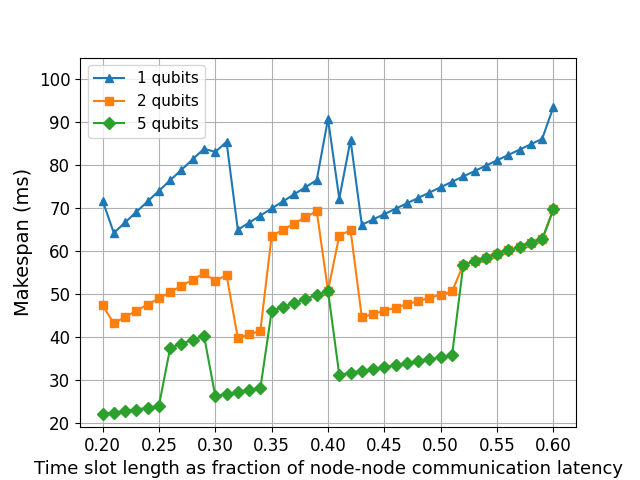
\includegraphics[width=1.0\columnwidth]{figures/qoala/teleport-self-preemption.png}
    \caption{Self-preemption of a teleportation program.
    For certain durations of the time slot length (as fraction of node-node communication latency, x-axis), the makespan is considerably higher (spikes in the plot).
    Reason: a classical message arrives for some teleportation instance $i$,
    making the node scheduler choose to perform the local quantum gates for $i$. During this,
    the time slot for instance $j > i$ starts. Since the QPS is busy with $i$, it cannot work on entanglement
    generation for $j$. Therefore, $j$ must wait for the next repetition of the network schedule, leading to a higher overall makespan.
    }
    \label{fig:teleport_self_preemption}
\end{figure}

\subsection{Demonstrating Qoala's multitasking potential}
Next, we demonstrate that Qoala can execute multiple instances of (different) programs concurrently by interleaving. We examine (1) makespan decrease (Section~\ref{sec:background_context}) when interleaving the instances compared to sequential execution, % (scheduling all instances in sequence).
(2) whether makespan depends on the network schedule.

We first evaluate multitasking instances of the same application: teleportation (same as A3 in \ref{sec:demonstrating_architecture_effectiveness}), 100 instances, with a fixed network schedule (no time slots; entanglement generation always allowed).
Sequential scheduling of instances results in makespan $N \cdot CC$
while interleaved scheduling (tasks for all instances created at the same time; no precedence constraints between instances) results in $\left\lceil N / Q \right\rceil \cdot CC$
(number of instances $N$, classical node-node communication latency $CC$, number of available memory qubits at receiving node $Q$).
We also evaluate the effect of network schedules with time slots (repeating pattern of slots assigned to A3 instances), and find that the time slots length influences the makespan (Figure~\ref{fig:teleport_self_preemption}) in a non-trivial manner due to instances pre-empting each other.
BQC (same as A2 in \ref{sec:demonstrating_architecture_effectiveness}, 100 instances) interleaved gives a makespan decrease over sequential of ($21\%, 56\%, 65\%$) for (2, 5, 10) server qubits, respectively.
The network schedule affects the makespan decrease: doubling the time slot length results in a smaller decrease ($12\%, 48\%, 48\%$). 

We then execute instances of different applications and again examine the effect of the network schedule on the makespan decrease: 50 QKD (A1 in \ref{sec:demonstrating_architecture_effectiveness}) and 50 BQC (A2) instances give a makespan decrease of $9.5\%$ (fixed schedule which first has time slots for QKD and then for BQC) and $39\%$ (schedule with time slots alternating between QKD and BQC).
We observe that multitasking can lead to improved (lower) makespan and that the network schedule can have considerable impact on the makespan.

\begin{figure}% [ht]
    \centering
    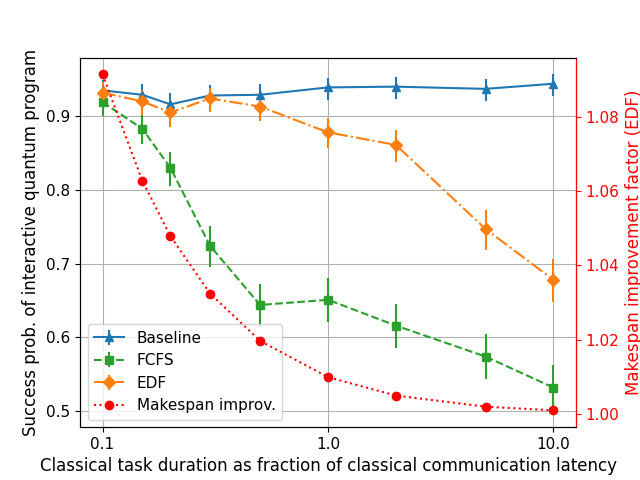
\includegraphics[width=1.0\columnwidth]{figures/qoala/tradeoffs_cq.png}
    \caption{Execution of interactive quantum program in the presence of a `busy' CPS program (tasks with duration $f \cdot CC$ for fraction $f$ of the classical node-to-node latency $CC$, x-axis).
    \textbf{Comparison of schedulers:}
    $Baseline$ (no scheduling nor interleaving),
    $FCFS$: first-come-first-serve scheduler (interleaving possible, no deadlines to prioritize quantum tasks),
    $EDF$: earliest-deadline-first scheduler (with deadlines to prioritize quantum tasks).
    The interactive program regularly waits (duration $CC$), with quantum states in memory, for incoming classical messages. % before continuing.
    Task interleaving allows busy CPS tasks to fill waiting times.
    EDF leads to higher success probability than FCFS, showcasing usefulness of deadlines.
    \textbf{Tradeoffs:}
    The baseline of sequential execution leads to the best possible success probability (quantum metric) at the expense of longest makespan. EDF allows a lowering of makespan (classical metric) at the expense of a lower succ. prob. (quantum metric). 
    % leads to the best succ. prob. since there is no interleaving (while qubits are in memory).
    %EDF succ. prob. lower than baseline is juxtaposed by an improvement (decrease) of makespan (improvement factor above 1, plotted on right axis as baseline makespan divided by EDF makespan).
    }
    \label{fig:eval_tradeoffs_cq}
\end{figure}

\subsection{Improvement over NetQASM architecture}
\label{sec:improvement_over_netqasm}
We compare the Qoala architecture with the NetQASM runtime approach for executing programs on a node from~\cite{dahlberg2022netqasm}
and show that Qoala provides new compilation possibilities (optimizing across classical and quantum code) and can lead to a better application execution makespan.
We consider a remote measurement-based quantum computing program written in Python (the program format of the NetQASM runtime) which has suboptimal code logic on purpose.
Executing this program in the NetQASM runtime performs worse (success probability $66\%$) than the same program but compiled manually into a Qoala program and executed in the Qoala runtime (succ. prob. $82\%$).
We note that manual compilation allowed optimization that is not possible in the NetQASM program format, exemplifying the new compilation potential provided by Qoala.

\begin{figure*}
    \newcommand{\heatmapheight}{6.6cm}
    \centering
    \subfloat[\centering \label{fig:heatmap_teleport}]{{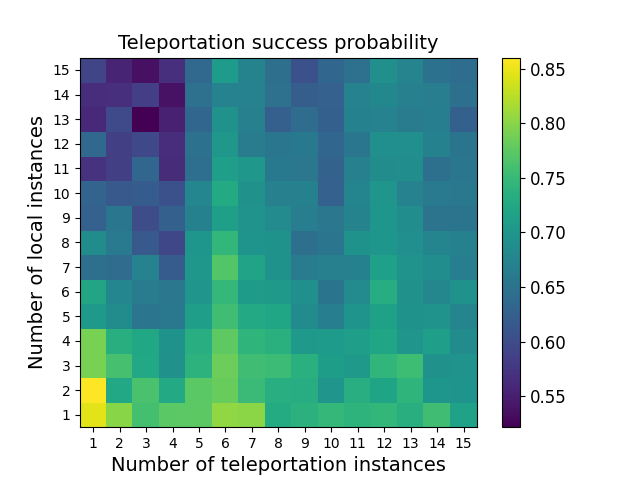
\includegraphics[height=\heatmapheight, keepaspectratio]{figures/qoala/heatmap_teleport.png}}}%
    \hfill
    \subfloat[\centering \label{fig:heatmap_local}]{{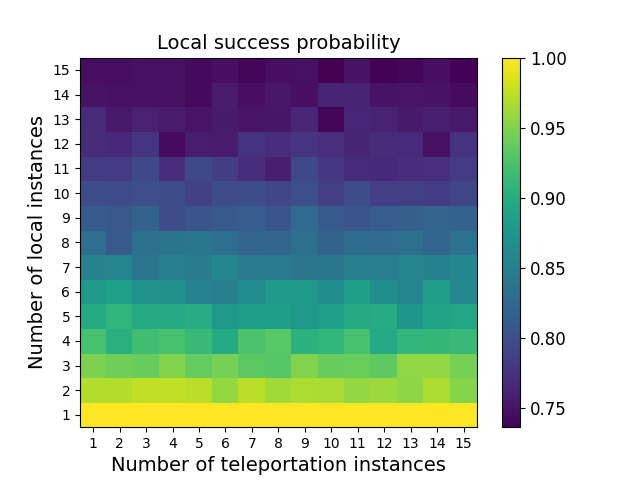
\includegraphics[height=\heatmapheight, keepaspectratio]{figures/qoala/heatmap_local.png}}}%
    \caption{
        Concurrent execution of teleportation (A3) and a local application (only preparing and measuring qubits).
        (a) Success probability of teleportation for different numbers of teleportation and local instances.
        More local instances lead to lower teleportation succ. prob. (effect more pronounced with few teleportation instances).
        (b) Success probability of local program. More local instances lead to lower local succ. prob., independent of the number of teleportation instances.}%
    \label{fig:quantum_multi_tasking}%
\end{figure*}


\subsection{Tradeoffs between classical and quantum performance metrics}
\label{sec:effectiveness_of_task_splitting}
We compare different scheduling modes enabled by Qoala and evaluate tradeoffs between makespan and success probability, noting that the NetQASM runtime did not allow scheduling at all (Figure~\ref{fig:eval_tradeoffs_cq}).
We expect that interleaving of tasks reduces the makespan, but may lead to lower success probability due qubits degrading in memory while tasks wait for each other.
We compare 3 scheduling modes: no scheduling (baseline), FCFS scheduling, and EDF scheduling.
We consider a simple runtime scenario with 
(1) a local quantum program which alternates between doing local quantum gates and waiting for a remote classical message before continuing and 
(2) a classical `busy program' consisting only of CPS tasks (duration defined as fraction of classical node-node latency).
We find that
(a) scheduling (FCFS or EDF) decreases success probability (EDF less than FCFS); impact larger for long task durations, but
(b) EDF provides a better makespan than no scheduling.
Note that the baseline necessarily gives the highest success probability due to no waiting, but at the expense of maximal makespan (sequential execution).

\subsection{Success probabilities with quantum multitasking}
\label{sec:quantum_multitasking}
Next, we consider a quantum multitasking scenario where we investigate trends in application success probability while varying the number of concurrent applications (Figure~\ref{fig:quantum_multi_tasking}).
In addition to a teleportation application (A3 in \ref{sec:demonstrating_architecture_effectiveness}), the receiver node also executes multiple instances of a local quantum program (only applying quantum gates).
Whenever the receiver node must wait for classical messages to come in for A3, it can work on its local quantum programs.
We find that success probability of both types of programs decreases in the presence of another program.

\subsection{Performance sensitivity}
Finally, we investigate the influence of classical message-passing latencies, internal latencies, and network schedule contents on application success probability of BQC (A2, 100 instances).
We find that the duration of sending classical messages between nodes has a large impact on the success probability:
node-node latencies [$0.01$, $0.1$, $1$] times the qubit coherence time lead to success probabilities [$0.89(2)$, $0.83(2)$, $0.54(4)$], respectively.
Internal latencies (between CPS and QPS, and between the scheduler and CPS or QPS) only have a significant impact when message-passing durations are low (0.01 times the qubit coherence time).
We also compare different network schedules (simple linear repeating schedule where each client-server pair gets a time slot consecutively; slot length is varied).
We obtain success probabilities [$0.90(2)$, $0.69(3)$, $0.48(4)$] for time slot lengths [$0.01$, $0.1$, $1$] times the qubit coherence time, respectively.
